\documentclass[]{book}
\usepackage{lmodern}
\usepackage{amssymb,amsmath}
\usepackage{ifxetex,ifluatex}
\usepackage{fixltx2e} % provides \textsubscript
\ifnum 0\ifxetex 1\fi\ifluatex 1\fi=0 % if pdftex
  \usepackage[T1]{fontenc}
  \usepackage[utf8]{inputenc}
\else % if luatex or xelatex
  \ifxetex
    \usepackage{mathspec}
  \else
    \usepackage{fontspec}
  \fi
  \defaultfontfeatures{Ligatures=TeX,Scale=MatchLowercase}
\fi
% use upquote if available, for straight quotes in verbatim environments
\IfFileExists{upquote.sty}{\usepackage{upquote}}{}
% use microtype if available
\IfFileExists{microtype.sty}{%
\usepackage{microtype}
\UseMicrotypeSet[protrusion]{basicmath} % disable protrusion for tt fonts
}{}
\usepackage[margin=1in]{geometry}
\usepackage{hyperref}
\hypersetup{unicode=true,
            pdftitle={Automated Gating of Flow Cytometry Data using the Bioconductor openCyto Framework},
            pdfauthor={Nichole Monhait, MPH Candidate; Colorado School of Public Health, Colorado State University},
            pdfborder={0 0 0},
            breaklinks=true}
\urlstyle{same}  % don't use monospace font for urls
\usepackage{natbib}
\bibliographystyle{plainnat}
\usepackage{color}
\usepackage{fancyvrb}
\newcommand{\VerbBar}{|}
\newcommand{\VERB}{\Verb[commandchars=\\\{\}]}
\DefineVerbatimEnvironment{Highlighting}{Verbatim}{commandchars=\\\{\}}
% Add ',fontsize=\small' for more characters per line
\usepackage{framed}
\definecolor{shadecolor}{RGB}{248,248,248}
\newenvironment{Shaded}{\begin{snugshade}}{\end{snugshade}}
\newcommand{\AlertTok}[1]{\textcolor[rgb]{0.94,0.16,0.16}{#1}}
\newcommand{\AnnotationTok}[1]{\textcolor[rgb]{0.56,0.35,0.01}{\textbf{\textit{#1}}}}
\newcommand{\AttributeTok}[1]{\textcolor[rgb]{0.77,0.63,0.00}{#1}}
\newcommand{\BaseNTok}[1]{\textcolor[rgb]{0.00,0.00,0.81}{#1}}
\newcommand{\BuiltInTok}[1]{#1}
\newcommand{\CharTok}[1]{\textcolor[rgb]{0.31,0.60,0.02}{#1}}
\newcommand{\CommentTok}[1]{\textcolor[rgb]{0.56,0.35,0.01}{\textit{#1}}}
\newcommand{\CommentVarTok}[1]{\textcolor[rgb]{0.56,0.35,0.01}{\textbf{\textit{#1}}}}
\newcommand{\ConstantTok}[1]{\textcolor[rgb]{0.00,0.00,0.00}{#1}}
\newcommand{\ControlFlowTok}[1]{\textcolor[rgb]{0.13,0.29,0.53}{\textbf{#1}}}
\newcommand{\DataTypeTok}[1]{\textcolor[rgb]{0.13,0.29,0.53}{#1}}
\newcommand{\DecValTok}[1]{\textcolor[rgb]{0.00,0.00,0.81}{#1}}
\newcommand{\DocumentationTok}[1]{\textcolor[rgb]{0.56,0.35,0.01}{\textbf{\textit{#1}}}}
\newcommand{\ErrorTok}[1]{\textcolor[rgb]{0.64,0.00,0.00}{\textbf{#1}}}
\newcommand{\ExtensionTok}[1]{#1}
\newcommand{\FloatTok}[1]{\textcolor[rgb]{0.00,0.00,0.81}{#1}}
\newcommand{\FunctionTok}[1]{\textcolor[rgb]{0.00,0.00,0.00}{#1}}
\newcommand{\ImportTok}[1]{#1}
\newcommand{\InformationTok}[1]{\textcolor[rgb]{0.56,0.35,0.01}{\textbf{\textit{#1}}}}
\newcommand{\KeywordTok}[1]{\textcolor[rgb]{0.13,0.29,0.53}{\textbf{#1}}}
\newcommand{\NormalTok}[1]{#1}
\newcommand{\OperatorTok}[1]{\textcolor[rgb]{0.81,0.36,0.00}{\textbf{#1}}}
\newcommand{\OtherTok}[1]{\textcolor[rgb]{0.56,0.35,0.01}{#1}}
\newcommand{\PreprocessorTok}[1]{\textcolor[rgb]{0.56,0.35,0.01}{\textit{#1}}}
\newcommand{\RegionMarkerTok}[1]{#1}
\newcommand{\SpecialCharTok}[1]{\textcolor[rgb]{0.00,0.00,0.00}{#1}}
\newcommand{\SpecialStringTok}[1]{\textcolor[rgb]{0.31,0.60,0.02}{#1}}
\newcommand{\StringTok}[1]{\textcolor[rgb]{0.31,0.60,0.02}{#1}}
\newcommand{\VariableTok}[1]{\textcolor[rgb]{0.00,0.00,0.00}{#1}}
\newcommand{\VerbatimStringTok}[1]{\textcolor[rgb]{0.31,0.60,0.02}{#1}}
\newcommand{\WarningTok}[1]{\textcolor[rgb]{0.56,0.35,0.01}{\textbf{\textit{#1}}}}
\usepackage{longtable,booktabs}
\usepackage{graphicx,grffile}
\makeatletter
\def\maxwidth{\ifdim\Gin@nat@width>\linewidth\linewidth\else\Gin@nat@width\fi}
\def\maxheight{\ifdim\Gin@nat@height>\textheight\textheight\else\Gin@nat@height\fi}
\makeatother
% Scale images if necessary, so that they will not overflow the page
% margins by default, and it is still possible to overwrite the defaults
% using explicit options in \includegraphics[width, height, ...]{}
\setkeys{Gin}{width=\maxwidth,height=\maxheight,keepaspectratio}
\IfFileExists{parskip.sty}{%
\usepackage{parskip}
}{% else
\setlength{\parindent}{0pt}
\setlength{\parskip}{6pt plus 2pt minus 1pt}
}
\setlength{\emergencystretch}{3em}  % prevent overfull lines
\providecommand{\tightlist}{%
  \setlength{\itemsep}{0pt}\setlength{\parskip}{0pt}}
\setcounter{secnumdepth}{5}
% Redefines (sub)paragraphs to behave more like sections
\ifx\paragraph\undefined\else
\let\oldparagraph\paragraph
\renewcommand{\paragraph}[1]{\oldparagraph{#1}\mbox{}}
\fi
\ifx\subparagraph\undefined\else
\let\oldsubparagraph\subparagraph
\renewcommand{\subparagraph}[1]{\oldsubparagraph{#1}\mbox{}}
\fi

%%% Use protect on footnotes to avoid problems with footnotes in titles
\let\rmarkdownfootnote\footnote%
\def\footnote{\protect\rmarkdownfootnote}

%%% Change title format to be more compact
\usepackage{titling}

% Create subtitle command for use in maketitle
\newcommand{\subtitle}[1]{
  \posttitle{
    \begin{center}\large#1\end{center}
    }
}

\setlength{\droptitle}{-2em}

  \title{Automated Gating of Flow Cytometry Data using the Bioconductor \texttt{openCyto} Framework}
    \pretitle{\vspace{\droptitle}\centering\huge}
  \posttitle{\par}
    \author{Nichole Monhait, MPH Candidate \\ Colorado School of Public Health, Colorado State University}
    \preauthor{\centering\large\emph}
  \postauthor{\par}
      \predate{\centering\large\emph}
  \postdate{\par}
    \date{2019-05-13}

\usepackage{booktabs}

\begin{document}
\maketitle

{
\setcounter{tocdepth}{1}
\tableofcontents
}
\hypertarget{whats-inside}{%
\chapter{What's inside?}\label{whats-inside}}

Flow cyometry is a method used to gain understanding of cell samples and populations by quantifying scattered and emitted fluorescent light. Signals are captured and analyzed through use of software programs. Flow cytometry analysis consists of gating, a method that dictates which cells will be further analyzed and which will not. Current methods for flow cytometry gating involve manually drawing gates. This process is both time consuming and costly, making automated gating procedures an appealing option. The \texttt{openCyto} package allows users to take manually gated data from flowJo, reproduce those gates in R, and eventually automate the gating process. The goal of this tutorial is to take the user through the process of automated gating analysis.

This tutorial will be useful to anyone who has done manual gating on a sample and wishes to automate the same procedure on additional samples in the future.

The example data used in this tutorial is from Colorado State University's Microbiology, Immunology, and Pathology Department. Alternatively, you can input your own data using the filetypes described in Chapter 3.

\hypertarget{getting-started}{%
\chapter{Getting Started}\label{getting-started}}

Here is an overview of the process to automate flow cytometry data using R's \texttt{openCyto} and what you will need to successfully automate your own flow cytometry analysis. The general steps to accomplish this are as follows:

\begin{enumerate}
\def\labelenumi{\arabic{enumi}.}
\tightlist
\item
  Read in a manually gated flowJo workspace in .wsp file format.
\item
  Parse raw FCS files from the read in workspace.
\item
  Visualize the manual gating template and resulting gates to verify gating scheme.
\item
  Create and read in a .csv gating template.
\item
  Automate gating.
\item
  Visualize automated gating template and gates to verify gating scheme.
\item
  Extract population statistics and relevant information.
\end{enumerate}

This process is completed primarily with the \texttt{openCyto} package but calls upon other packages within the \href{http://bioconductor.org/packages/release/bioc/html/openCyto.html}{Bioconductor} \texttt{openCyto} framework. Packages needed to complete this tutorial are listed at the end of this chapter. Descriptions of each function and R object used for this analysis are below.

\hypertarget{required-packages-and-installation}{%
\section{Required Packages and Installation}\label{required-packages-and-installation}}

\hypertarget{package-descriptions}{%
\subsection{Package descriptions}\label{package-descriptions}}

Below is a description of each package used in this analysis. Code to install and use these packages will follow. Package descriptions taken from Bioconductor and CRAN.

\begin{tabular}{c|c}
\hline
Package Name & Use\\
\hline
openCyto & This package is designed to facilitate the automated gating methods in sequential way to mimic the manual gating strategy.\\
\hline
flowWorkspace & This package allows you to import basic flowJo workspaces into BioConductor and replicate the gating from flowJo using the flowCore functionality. Gating hierarchies, groups of samples, compensation, and transformation are performed so that the output matches the flowJo analysis.\\
\hline
flowCore & Provides S4 data structures and basic functions to deal with flow cytometry data.\\
\hline
flowStats & Methods and functionality to analyse flow data that is beyond the basic infrastructure provided by the flowCore package.\\
\hline
flowClust & Robust model-based clustering using a t-mixture model with Box-Cox transformation.\\
\hline
data.table & Fast aggregation of large data (e.g. 100GB in RAM), fast ordered joins, fast add/modify/delete of columns by group using no copies at all, list columns, friendly and fast character-separated-value read/write. Offers a natural and flexible syntax, for faster development.\\
\hline
\end{tabular}

\hypertarget{installation}{%
\subsection{Installation}\label{installation}}

Install the following libraries into a new R script. As you will see below, this tutorial uses the development version of \texttt{openCyto}. It is important to use the development version of \texttt{openCyto} to remain up to date on any changes made by the developers of \texttt{openCyto}. Use the following to ensure the correct packages are installed. Installation will only need to be done once.

\emph{To install}

\begin{Shaded}
\begin{Highlighting}[]
\ControlFlowTok{if}\NormalTok{ (}\OperatorTok{!}\KeywordTok{requireNamespace}\NormalTok{(}\StringTok{"BiocManager"}\NormalTok{, }\DataTypeTok{quietly =} \OtherTok{TRUE}\NormalTok{))}
    \KeywordTok{install.packages}\NormalTok{(}\StringTok{"BiocManager"}\NormalTok{)}
\NormalTok{BiocManager}\OperatorTok{::}\KeywordTok{install}\NormalTok{() }

\NormalTok{BiocManager}\OperatorTok{::}\KeywordTok{install}\NormalTok{(}\KeywordTok{c}\NormalTok{(}\StringTok{"openCyto"}\NormalTok{, }\StringTok{"flowWorkspace"}\NormalTok{, }\StringTok{"flowCore"}\NormalTok{,}
                       \StringTok{"flowStats"}\NormalTok{, }\StringTok{"flowClust"}\NormalTok{))}

\KeywordTok{install.packages}\NormalTok{(}\StringTok{"data.table"}\NormalTok{)}
\NormalTok{devtools}\OperatorTok{::}\KeywordTok{install_github}\NormalTok{(}\StringTok{"RGLab/openCyto"}\NormalTok{, }\DataTypeTok{ref =} \StringTok{"trunk"}\NormalTok{)}
\end{Highlighting}
\end{Shaded}

RStudio may also prompt you to download \href{https://www.xquartz.org/}{XQuartz} and \href{https://developer.apple.com/xcode/}{XCode} based on your computer type, so it may be a good idea to go ahead and also download both.

\hypertarget{load-packages}{%
\subsection{Load packages}\label{load-packages}}

Although installation only needs to be done once, packages will need to be reloaded each time you open an R session. At the beginning of each session, run the following code.

\emph{To load}

\begin{Shaded}
\begin{Highlighting}[]
\KeywordTok{library}\NormalTok{(openCyto)}
\KeywordTok{library}\NormalTok{(flowWorkspace)}
\KeywordTok{library}\NormalTok{(data.table)}
\KeywordTok{library}\NormalTok{(flowCore)}
\KeywordTok{library}\NormalTok{(flowStats)}
\KeywordTok{library}\NormalTok{(flowClust)}
\end{Highlighting}
\end{Shaded}

\hypertarget{working-with-your-manual-gating-scheme}{%
\chapter{Working with your Manual Gating Scheme}\label{working-with-your-manual-gating-scheme}}

The first step in this process is to bring a pre-existing flowJo file into R in order to recreate the gating environment. The remainder of this chapter will detail the following:

\begin{enumerate}
\def\labelenumi{\arabic{enumi}.}
\tightlist
\item
  Read in flowJo .wsp file\\
\item
  Parse FCS files\\
\item
  Visualize and verify manual gates
\end{enumerate}

\hypertarget{read-in-flowjo-file}{%
\section{Read in flowJo file}\label{read-in-flowjo-file}}

Within flowJo, tranformation, compensation, and gating can be saved as either \emph{.xml} or \emph{.wsp} filetypes. This tutorial will only detail steps from a \emph{.wsp} filetype saved from flowJo. Note that many other tutorials begin from a \emph{.xml} filetype. Saving analysis within flowJo is detailed \href{http://docs.flowjo.com/vx/workspaces-and-samples/ws-savinganalysis/}{here}. Your \emph{.wsp} file will contain samples and groups to be added to the Workspace in R, all gates and analyses, and compensation matrices. Importantly, the \emph{.wsp} will not save your FCS files. Rather, the path to your files will be saved and can be adjusted later within R.

Before you begin, be sure you have loaded the required packages outlined in the previous chapter.

Once all packages are loaded, save the \emph{.wsp} file path as an R object called \textbf{wsfile}. Next, use \texttt{openWorkspace()} with your R object created in the prior step to open the \emph{.wsp} file in R. Save this as an R object. Here, this was saved as \textbf{ws} and is of flowJoWorkspace class. Here is an example of saving and opening your \emph{.wsp} filetype in R. Please ensure that \textbf{ws} is saved as a flowWorkspace object containing groups of samples before proceeding.

\begin{Shaded}
\begin{Highlighting}[]
\NormalTok{wsfile <-}\StringTok{ "./tutorial/group1_v_group2.wsp"}
\end{Highlighting}
\end{Shaded}

\begin{Shaded}
\begin{Highlighting}[]
\NormalTok{ws <-}\StringTok{ }\KeywordTok{openWorkspace}\NormalTok{(wsfile)}
\end{Highlighting}
\end{Shaded}

\begin{Shaded}
\begin{Highlighting}[]
\KeywordTok{print}\NormalTok{(ws)}
\end{Highlighting}
\end{Shaded}

\begin{verbatim}
## FlowJo Workspace Version  20.0 
## File location:  ./tutorial 
## File name:  group1_v_group2.wsp 
## Workspace is open. 
## 
## Groups in Workspace
##          Name Num.Samples
## 1 All Samples          10
## 2     Samples          10
\end{verbatim}

\hypertarget{parse-fcs-files}{%
\section{Parse FCS files}\label{parse-fcs-files}}

The next step is to read in raw FCS files. FCS files contain data from the cytometer. Standards for FCS files are listed \href{http://software.broadinstitute.org/cancer/software/genepattern/attachments/fcs_3_1_standard.pdf}{here}.

Raw FCS files are read using the \texttt{parseWorkspace} function. This function will read the FCS files and transform, compensate, and gate according to parameters defined from the \emph{.wsp} flowJo workspace, which is now saved as an R object of class flowWorkspace. The \texttt{parseWorkspace} call requires the object that results from running \texttt{openWorkspace}. Here, we named this object \texttt{ws}. The function \texttt{parseWorkspace()} also requires the name of the samples to read in. To list sample names, use the \texttt{getSampleGroups()} function on your flowWorkspace class object. Other options may be customized based on particular needs. A new R object named \texttt{gating\_set} is then created and will be a GatingSet object. The \texttt{isNcdf\ =\ TRUE} call saves this output to disk rather that into memory because the files are large. Here is an example of parsing FCS files. As this function runs, you will see several messages appear as the FCS files are loaded and the manual gating scheme is replicated. After this, \texttt{attributes()} is used to examine the data.

\begin{Shaded}
\begin{Highlighting}[]
\NormalTok{gating_set <-}\StringTok{ }\KeywordTok{parseWorkspace}\NormalTok{(ws, }\DataTypeTok{name =} \StringTok{"Samples"}\NormalTok{, }\DataTypeTok{path =} \StringTok{"./tutorial/group1_v_group2"}\NormalTok{, }\DataTypeTok{isNcdf =} \OtherTok{TRUE}\NormalTok{, }\DataTypeTok{sampNloc =} \StringTok{'sampleNode'}\NormalTok{)}
\end{Highlighting}
\end{Shaded}

\begin{verbatim}
## windows version of flowJo workspace recognized.
## version X
\end{verbatim}

\begin{Shaded}
\begin{Highlighting}[]
\KeywordTok{attributes}\NormalTok{(gating_set)}
\end{Highlighting}
\end{Shaded}

\hypertarget{visualize-and-verify}{%
\section{Visualize and Verify}\label{visualize-and-verify}}

It is helpful to now visualize both the gating template and gates on a subset of the data in order to verify the gating scheme. This will ensure consistency between the flowJo workspace and the manual gates recreated in R. First, save a subset of the \texttt{gating\_set} as follows. The following saves the first FCS file of \textbf{gating\_set} as \textbf{gh}. Since each FCS file corresponds to an individual experiment, this saves the first experiment of the group.

\begin{Shaded}
\begin{Highlighting}[]
\NormalTok{gh <-}\StringTok{ }\NormalTok{gating_set[[}\DecValTok{1}\NormalTok{]]}
\KeywordTok{print}\NormalTok{(gh)}
\end{Highlighting}
\end{Shaded}

\begin{verbatim}
## Sample:  X_group1_1 
## GatingHierarchy with  51  gates
\end{verbatim}

\hypertarget{plot}{%
\subsection{plot()}\label{plot}}

The plot() function will visualize the current gating hierarchy when applied to an object of class GatingHierarchy. This can be done for the entire gating hierarchy or a specific population as seen below.

\begin{Shaded}
\begin{Highlighting}[]
\KeywordTok{plot}\NormalTok{(gh)}
\end{Highlighting}
\end{Shaded}

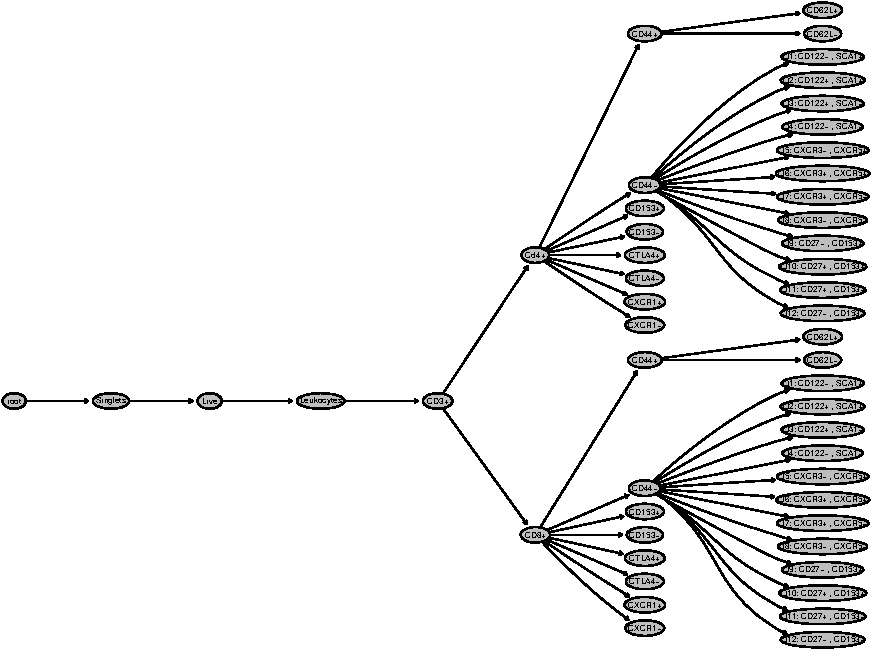
\includegraphics{bookdown_autogating_files/figure-latex/manual_hierarchy-1.pdf}

\hypertarget{plotgate}{%
\subsection{plotGate()}\label{plotgate}}

The plotGate() function will gate the designated subset of your data according to parameters replicated from flowJo. This must also be called on an object of class GatingHierarchy.

\begin{Shaded}
\begin{Highlighting}[]
\KeywordTok{flowWorkspace.par.set}\NormalTok{(}\StringTok{"plotGate"}\NormalTok{, }\KeywordTok{list}\NormalTok{(}\DataTypeTok{xlim =} \StringTok{"data"}\NormalTok{,}
                                       \DataTypeTok{ylim =} \StringTok{"data"}\NormalTok{))}
\KeywordTok{plotGate}\NormalTok{(gh)}
\end{Highlighting}
\end{Shaded}

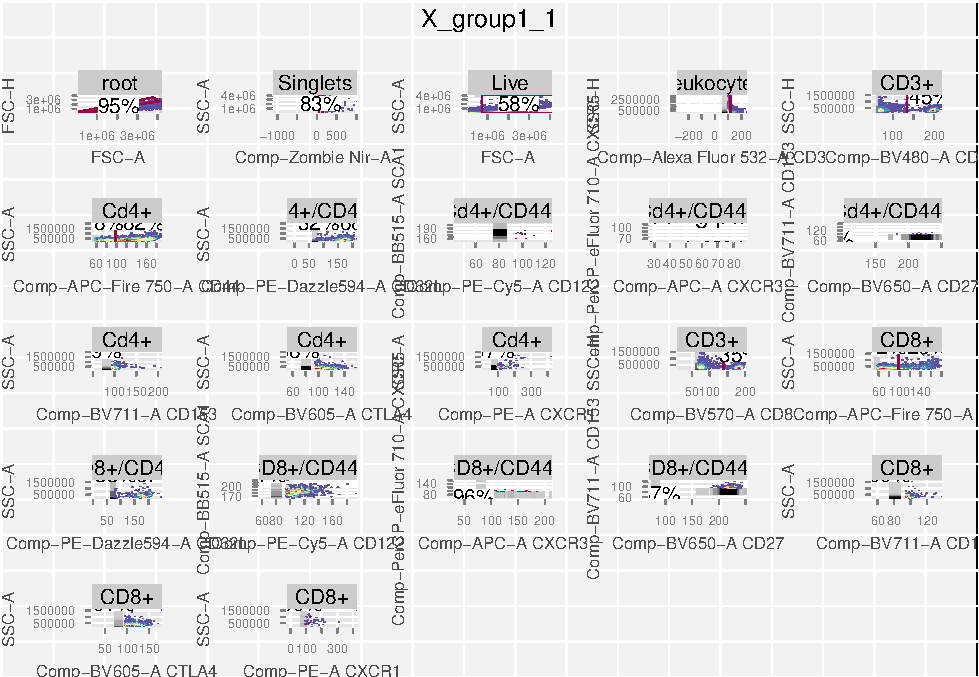
\includegraphics{bookdown_autogating_files/figure-latex/visualize_subset-1.pdf}

**Note the use of \texttt{flowWorkspace.par.set()} here. Chapter 5 of this tutorial will discuss customizations such as this one.

\hypertarget{create-.csv}{%
\chapter{Create .csv}\label{create-.csv}}

The creation of a .csv gating template is arguably the most important step to automating flow cytometry analysis. The .csv template that you create will tell \texttt{openCyto} how to gate your data. Included with this tutorial is a partial .csv template that can be used to gate the sample data. Generally, .csv templates will look like this:

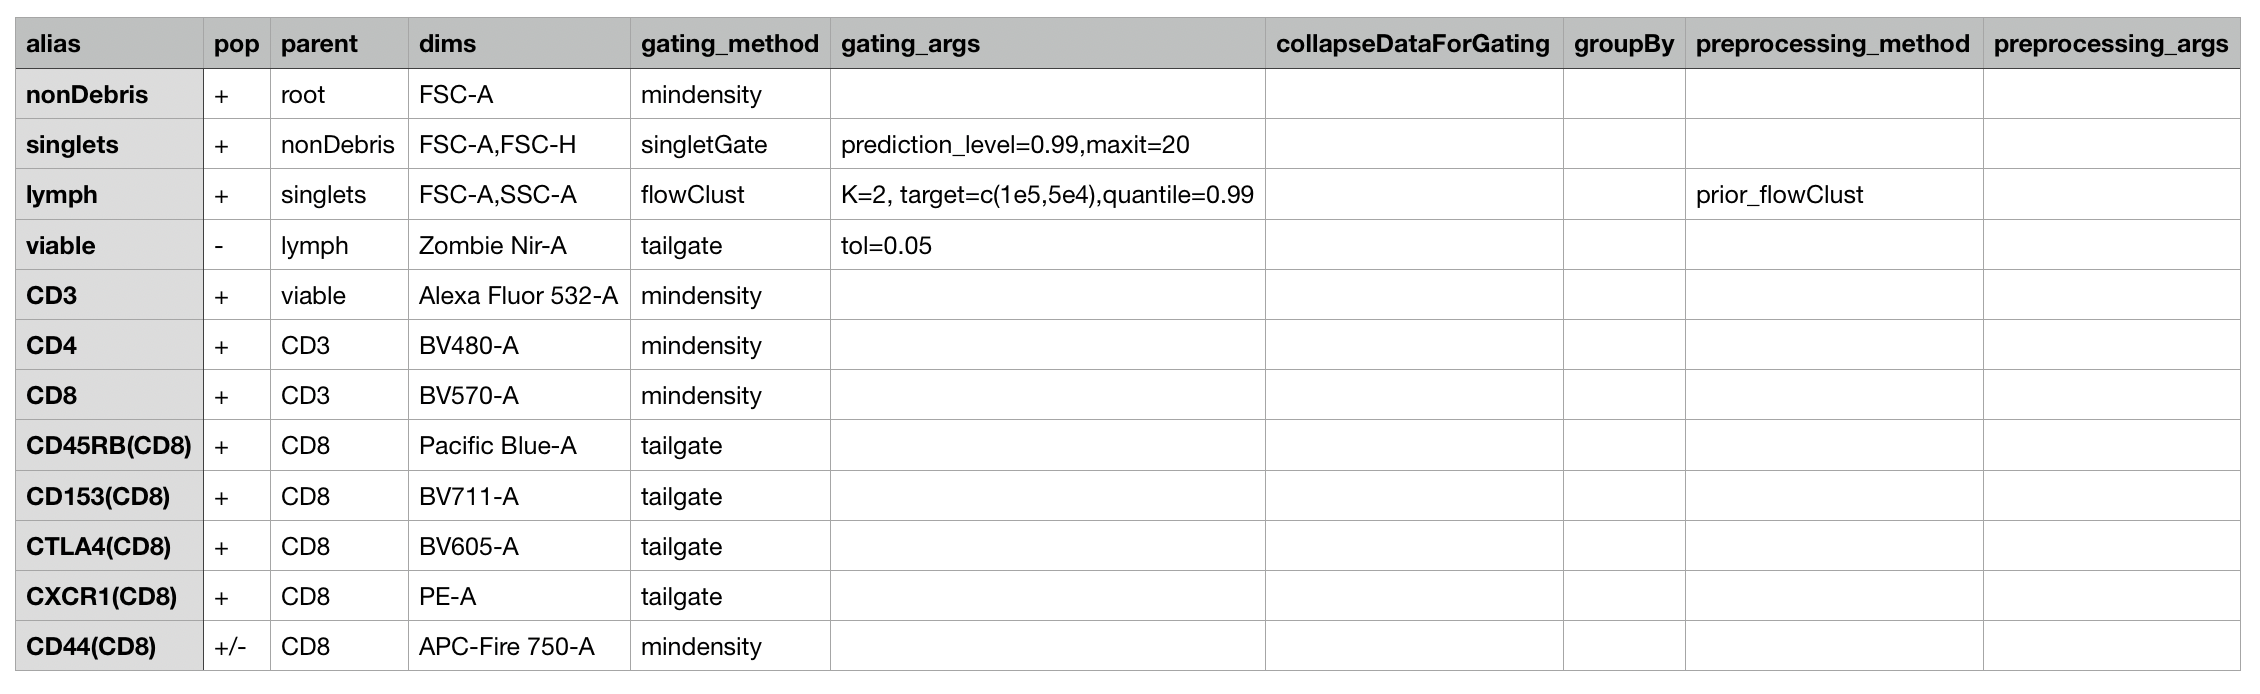
\includegraphics[width=0.6\linewidth]{/Users/monhait/Desktop/data/images/entire_csv}

\hypertarget{csv-gating-template-structure}{%
\section{.csv Gating Template Structure}\label{csv-gating-template-structure}}

In the gating template, each row corresponds to a single cell population and the method used to gate that population. When read into R, the .csv will direct gating based on parameters listed in each row and column. The .csv must contain 10 predefined columns as seen here:

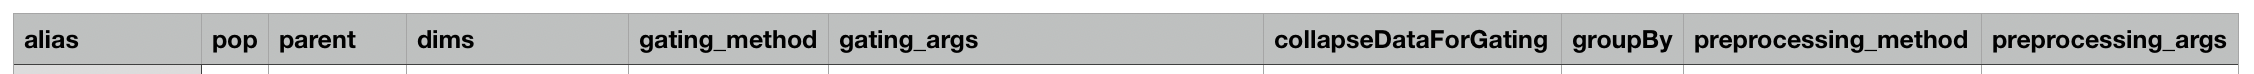
\includegraphics[width=0.6\linewidth]{/Users/monhait/Desktop/data/images/cols}

\hypertarget{alias}{%
\subsection{\texorpdfstring{\texttt{alias}}{alias}}\label{alias}}

The first column must be titled \texttt{alias}. This is where you will put your cell population names. Remember, each row corresponds to a single cell population. Population names in the \texttt{alias} column must be unique.

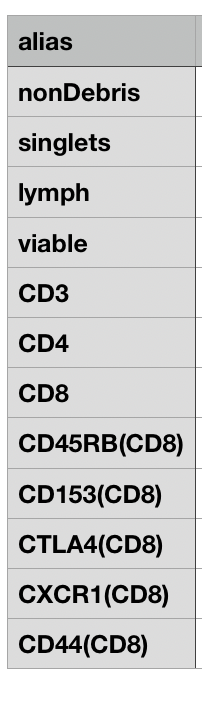
\includegraphics[width=0.6\linewidth]{/Users/monhait/Desktop/data/images/alias}

\hypertarget{pop}{%
\subsection{\texorpdfstring{\texttt{pop}}{pop}}\label{pop}}

The second column must be titled \texttt{pop}. This column will contain a \texttt{+} or \texttt{-} to designate which subset or quadrant will be gated. A \texttt{+} will gate the positive subset while a \texttt{-} will gate the negative. This column can only contain strings of \texttt{+} and \texttt{-}, so do not use any characters as separators for quadrant gates.

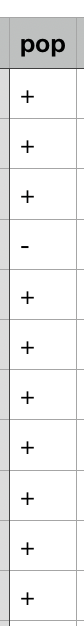
\includegraphics[width=0.6\linewidth]{/Users/monhait/Desktop/data/images/pop}

\hypertarget{parent}{%
\subsection{\texorpdfstring{\texttt{parent}}{parent}}\label{parent}}

The third column must be titled \texttt{parent}. This column refers to the parent cell population, or where the current cell population originates from. Similar to the \texttt{alias} column, \texttt{parent} names must be unique. This column cannot contain any commas, otherwise \texttt{openCyto} will assume the population has multiple parents and you will get an error message.

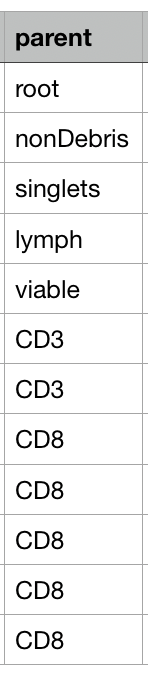
\includegraphics[width=0.6\linewidth]{/Users/monhait/Desktop/data/images/parent}

\hypertarget{remaining-template-columns}{%
\subsection{Remaining template columns}\label{remaining-template-columns}}

\texttt{dims}- channel or marker names for gating\\
\texttt{gating\_method}- gating function (supported options listed above)\\
quadrantGate\\
rangeGate\\
quantileGate\\
mindensity\\
tailgate\\
cytokine\\
flowClust\\
boundary\\
singletGate\\
transitional\\
plolyfunctionalityGate\\
flowDensity
\texttt{gating\_args}- arguments to be passed to gating function
\texttt{collapseDataforGating}- data is collapsed and replicated across all samples\\
\texttt{groupBy}- used to group samples into unique combinations\\
\texttt{preprocessing\_method}- preprocessing function\\
\texttt{preprocessing\_args}- arguments for preprocessing function

\hypertarget{creating-the-template}{%
\section{Creating the Template}\label{creating-the-template}}

The gating template can be created manually or assisted by the use of the \texttt{templateGen()} function. The function \texttt{templateGen()} will input the \texttt{alias}, \texttt{pop}, \texttt{parent}, and \texttt{dims} columns and the rest must be completed manually. To use \texttt{templateGen()}, you must input a GatingHierarchy object. In this example, that is \textbf{gh}, the subset created from \textbf{gating\_set}.

\begin{Shaded}
\begin{Highlighting}[]
\NormalTok{gt <-}\StringTok{ }\KeywordTok{templateGen}\NormalTok{(gh)}
\KeywordTok{head}\NormalTok{(gt)}
\end{Highlighting}
\end{Shaded}

\begin{verbatim}
##        alias        pop                              parent
## 1   Singlets   Singlets                                root
## 2       Live       Live                           /Singlets
## 3 Leukocytes Leukocytes                      /Singlets/Live
## 4       CD3+       CD3+           /Singlets/Live/Leukocytes
## 5       CD8+       CD8+      /Singlets/Live/Leukocytes/CD3+
## 6     CXCR1-     CXCR1- /Singlets/Live/Leukocytes/CD3+/CD8+
##                           dims gating_method gating_args
## 1                  FSC-A,FSC-H          <NA>        <NA>
## 2            Comp-Zombie Nir-A          <NA>        <NA>
## 3                  FSC-A,SSC-A          <NA>        <NA>
## 4 Comp-Alexa Fluor 532-A,SSC-H          <NA>        <NA>
## 5           Comp-BV570-A,SSC-H          <NA>        <NA>
## 6                    Comp-PE-A          <NA>        <NA>
##   collapseDataForGating groupBy preprocessing_method preprocessing_args
## 1                  <NA>    <NA>                 <NA>               <NA>
## 2                  <NA>    <NA>                 <NA>               <NA>
## 3                  <NA>    <NA>                 <NA>               <NA>
## 4                  <NA>    <NA>                 <NA>               <NA>
## 5                  <NA>    <NA>                 <NA>               <NA>
## 6                  <NA>    <NA>                 <NA>               <NA>
\end{verbatim}

The auto-filled template will generate within the R Console and can then be saved locally with the following code. You will see that all columns besides the first four will contain NA values. These are the values that must be manually input to complete the .csv.

\begin{Shaded}
\begin{Highlighting}[]
\KeywordTok{write.csv}\NormalTok{(gt, }\StringTok{"gt.csv"}\NormalTok{)}
\end{Highlighting}
\end{Shaded}

If you choose to create the gating template manually, the same conventions must be followed. Start with a blank spreadsheet. Next, fill in the 10 required column names. From there, use the manual gating hierarchy to fill in each cell population \texttt{alias}. Fill in the remainder accordingly.

There will likely be troubleshooting involved in this process. \href{https://www.bioconductor.org/packages/devel/bioc/vignettes/openCyto/inst/doc/HowToWriteCSVTemplate.html\#14_gating_method_that_generates_multiple_populations}{This} is a great place to start if you're seeking more information on the gating template. The \texttt{openCyto} \href{https://github.com/RGLab/openCyto}{GitHub page} is also very responsive to issues posted.

\hypertarget{automate-gating}{%
\chapter{Automate Gating}\label{automate-gating}}

\hypertarget{load-.csv-into-r}{%
\section{Load .csv into R}\label{load-.csv-into-r}}

As noted in the previous chapter, there is a sample gating template titled \emph{partial.csv} with the sample data. This may serve as a guide to creating your own. When the .csv gating template is complete, it is then read into R and saved as \textbf{gt}, a gatingTemplate object.

\begin{Shaded}
\begin{Highlighting}[]
\NormalTok{gt <-}\StringTok{ }\KeywordTok{gatingTemplate}\NormalTok{(}\StringTok{"./tutorial/partial_gt.csv"}\NormalTok{)}
\end{Highlighting}
\end{Shaded}

The flow cytometry equipment at CSU will compensate and transform the data automatically. Other tutorials may highlight the steps to compensate and transform data, but these are not relevant to CSU at this moment. In the event that equipment changes, it may be necessary to complete compensation and transformation steps to prepare data. More on the current equipment used as CSU \href{https://www.umassmed.edu/facslab/instrument/core-cytek-aurora2/}{here}.

\hypertarget{read-in-raw-fcs-files}{%
\section{Read in raw FCS files}\label{read-in-raw-fcs-files}}

Now that the GatingTemplate object has been loaded into R, you will need to load in raw FCS files to perform the automated gating on. For gating, these files must be in a GatingSet object type, which requires the following steps. When the path is saved using \texttt{list.files}, a character matrix of file names will be saved. Next, \texttt{read.ncdfFlowSet} will save FCS files as a ncdfFlowSet obect. The \texttt{GatingSet} function will then save the FCS files as a GatingSet object. In this form, the FCS files can be input and gated.

\begin{Shaded}
\begin{Highlighting}[]
\NormalTok{fcs_files <-}\StringTok{ }\KeywordTok{list.files}\NormalTok{(}\DataTypeTok{path =} \StringTok{"./tutorial/group1_v_group2"}\NormalTok{, }\DataTypeTok{full.names =} \OtherTok{TRUE}\NormalTok{)}
\NormalTok{ncfs  <-}\StringTok{ }\KeywordTok{read.ncdfFlowSet}\NormalTok{(}\DataTypeTok{files =}\NormalTok{ fcs_files)}
\NormalTok{gs_auto <-}\StringTok{ }\KeywordTok{GatingSet}\NormalTok{(ncfs)}
\end{Highlighting}
\end{Shaded}

\hypertarget{apply-gating}{%
\section{Apply Gating}\label{apply-gating}}

At this point, you now have GatingTemplate and GatingSet object to be used for gating. Apply your GatingTemplate object to the GatingSet object, where x = GatingTemplate object and y = GatingSet object.

\begin{Shaded}
\begin{Highlighting}[]
\KeywordTok{gating}\NormalTok{(}\DataTypeTok{x =}\NormalTok{ gt, }\DataTypeTok{y =}\NormalTok{ gs_auto)}
\end{Highlighting}
\end{Shaded}

\hypertarget{plot-automated-gating}{%
\section{Plot Automated Gating}\label{plot-automated-gating}}

Just as before, plot both the gating hierarchy and the automated gates. You may notice extra nodes have been added to the hierarchy. Chapter 5 will highlight additional cusomization to remove unwanted nodes and improve upon visualization.

\begin{Shaded}
\begin{Highlighting}[]
\KeywordTok{plotGate}\NormalTok{(gs_auto[[}\DecValTok{1}\NormalTok{]])}
\end{Highlighting}
\end{Shaded}

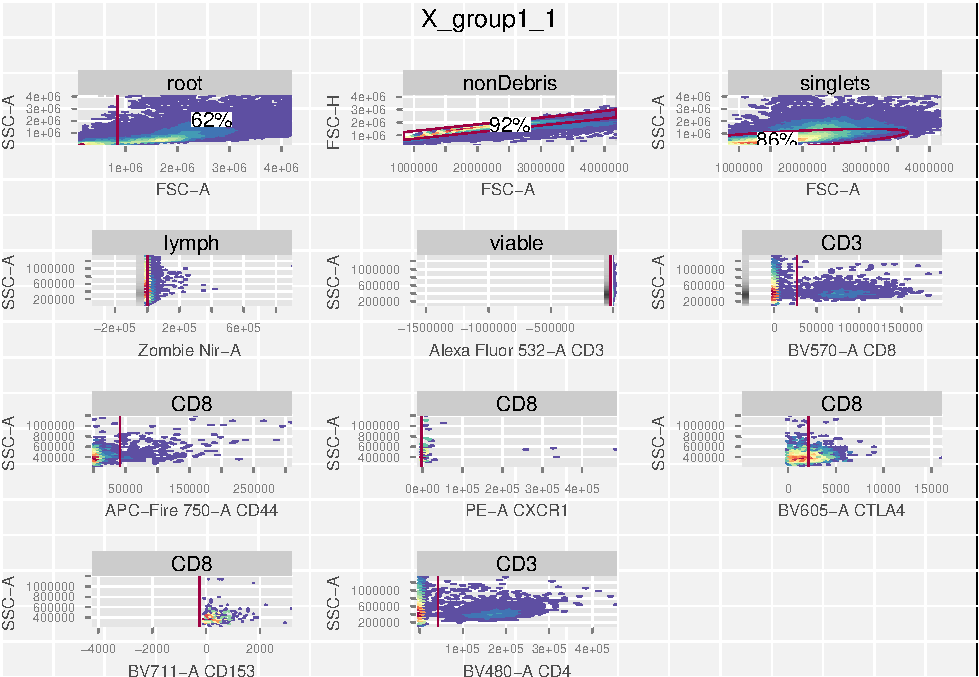
\includegraphics{bookdown_autogating_files/figure-latex/plot_auto_gates-1.pdf}

\begin{Shaded}
\begin{Highlighting}[]
\KeywordTok{plot}\NormalTok{(gs_auto[[}\DecValTok{1}\NormalTok{]])}
\end{Highlighting}
\end{Shaded}

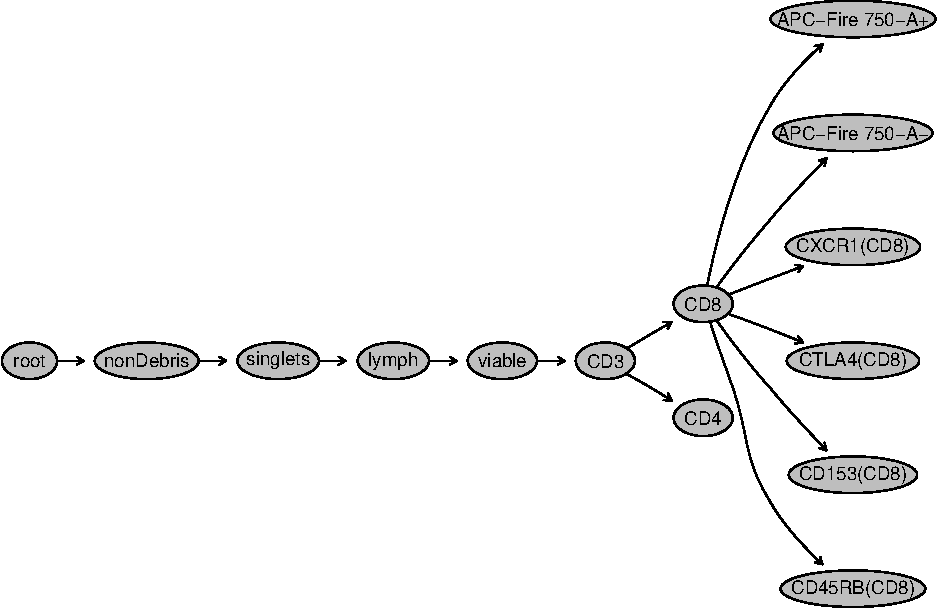
\includegraphics{bookdown_autogating_files/figure-latex/plot_auto_hierarchy-1.pdf}

\hypertarget{population-statistics}{%
\section{Population Statistics}\label{population-statistics}}

Both counts and frequencies can be generated for analysis. This can be generate based on the analysis completed in R, or pulled directly from flowJo. To pull from flowJo, simply at \texttt{flowJo=TRUE} to either code chunk below.

\textbf{Counts}

\begin{Shaded}
\begin{Highlighting}[]
\KeywordTok{head}\NormalTok{(}\KeywordTok{getPopStats}\NormalTok{(gs_auto,}\DataTypeTok{statistic=}\StringTok{"count"}\NormalTok{))}
\end{Highlighting}
\end{Shaded}

\begin{verbatim}
##          name Population    Parent Count ParentCount
## 1: X_group1_1  nonDebris      root 87715      142158
## 2: X_group1_1   singlets nonDebris 80775       87715
## 3: X_group1_1      lymph  singlets 69722       80775
## 4: X_group1_1     viable     lymph 40989       69722
## 5: X_group1_1        CD3    viable 40944       40989
## 6: X_group1_1        CD8       CD3  1888       40944
\end{verbatim}

\textbf{Frequencies}

\begin{Shaded}
\begin{Highlighting}[]
\KeywordTok{head}\NormalTok{(}\KeywordTok{getPopStats}\NormalTok{(gs_auto,}\DataTypeTok{statistic=}\StringTok{"freq"}\NormalTok{))}
\end{Highlighting}
\end{Shaded}

\begin{verbatim}
##          name Population    Parent Count ParentCount
## 1: X_group1_1  nonDebris      root 87715      142158
## 2: X_group1_1   singlets nonDebris 80775       87715
## 3: X_group1_1      lymph  singlets 69722       80775
## 4: X_group1_1     viable     lymph 40989       69722
## 5: X_group1_1        CD3    viable 40944       40989
## 6: X_group1_1        CD8       CD3  1888       40944
\end{verbatim}

\hypertarget{customization}{%
\chapter{Customization}\label{customization}}

It is possible that additional customization may be necessary when working with the \texttt{openCyto} framework. Below are three common customizations that will be outlined in this chapter.

\begin{enumerate}
\def\labelenumi{\arabic{enumi}.}
\tightlist
\item
  Hiding unwanted nodes
\item
  Renaming nodes
\item
  Adjusting plots
\end{enumerate}

\hypertarget{hiding-unwanted-nodes}{%
\section{Hiding unwanted nodes}\label{hiding-unwanted-nodes}}

When automating analysis, there may be nodes that were not predefined in the .csv gating template or nodes that may not be of interest in your particular analysis. Plotting the gating hierarchy using the \texttt{plot()} function will display this and then nodes can be hidden based on need with the following code. Below is an example of a ``full'' gating hierarchy and then the same hierarchy with the CD3+ node removed.

\textbf{Full Hierarchy}

\begin{Shaded}
\begin{Highlighting}[]
\KeywordTok{plot}\NormalTok{(gh)}
\end{Highlighting}
\end{Shaded}

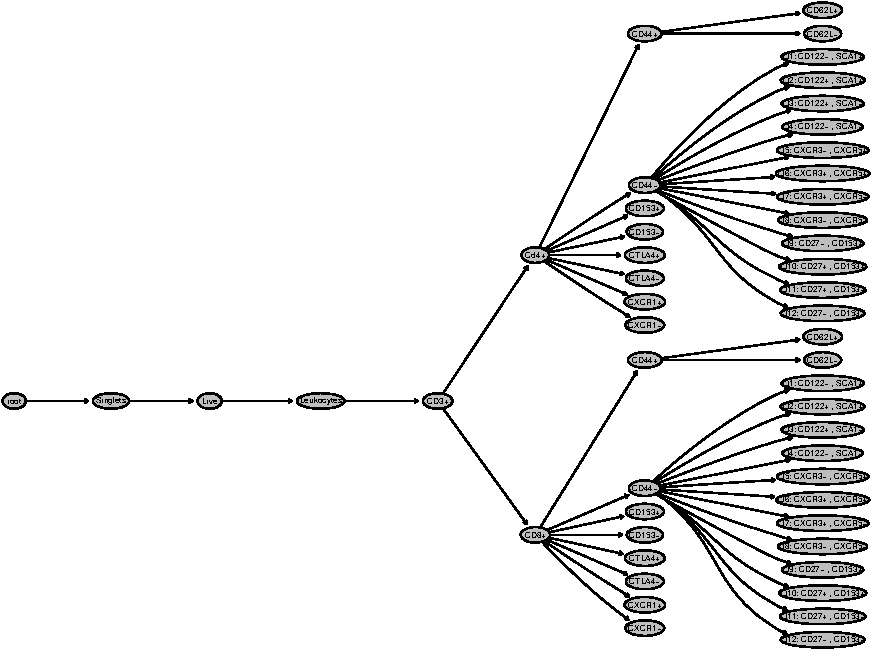
\includegraphics{bookdown_autogating_files/figure-latex/full_nodes-1.pdf}

\textbf{CD3+ Removed Hierarchy}

To remove nodes, first save the unwanted nodes as an R object named \textbf{nodesToHide}. Next, use the code following the \texttt{lapply()} function, only replacing \textbf{gs} with your GatingSet object name.

\begin{Shaded}
\begin{Highlighting}[]
\NormalTok{nodesToHide <-}\StringTok{ "CD3+"}
\KeywordTok{lapply}\NormalTok{(nodesToHide, }\ControlFlowTok{function}\NormalTok{(thisNode)}\KeywordTok{setNode}\NormalTok{(gh, thisNode, }\OtherTok{FALSE}\NormalTok{))}
\end{Highlighting}
\end{Shaded}

\begin{verbatim}
## [[1]]
## NULL
\end{verbatim}

\hypertarget{renaming-nodes}{%
\section{Renaming nodes}\label{renaming-nodes}}

Rename nodes based on your preferences with the following code. Within the \texttt{setNode} function, the first input is the current cell population name and the second is the desired change.

\begin{Shaded}
\begin{Highlighting}[]
\KeywordTok{setNode}\NormalTok{(}\StringTok{"Live"}\NormalTok{, }\StringTok{"Viable"}\NormalTok{)}
\KeywordTok{plot}\NormalTok{(gh)}
\end{Highlighting}
\end{Shaded}

\hypertarget{adjusting-plots}{%
\section{Adjusting plots}\label{adjusting-plots}}

\hypertarget{adjust-plot-axes}{%
\subsection{Adjust plot axes}\label{adjust-plot-axes}}

As seen in chapter 2, it may be necessary to adjust the plot axes in order to best view the gates. This is done using the code below. Setting xlim and ylim to ``data'' adjusts plot based on the actual data range, rather than instrument specifications. Custom ranges can also be input numerically.

\begin{Shaded}
\begin{Highlighting}[]
\KeywordTok{flowWorkspace.par.set}\NormalTok{(}\StringTok{"plotGate"}\NormalTok{, }\KeywordTok{list}\NormalTok{(}\DataTypeTok{xlim =} \StringTok{"data"}\NormalTok{,}
                                       \DataTypeTok{ylim =} \StringTok{"data"}\NormalTok{))}
\end{Highlighting}
\end{Shaded}

Here is a comparison of xlim and ylim set as ``instrument'' and then ``data''.

\textbf{Instrument}

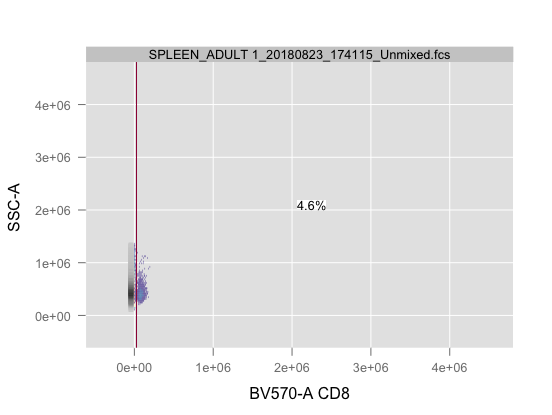
\includegraphics[width=0.6\linewidth]{/Users/monhait/Desktop/bookdown_autogating/images/CD8_instrument}

\textbf{Data}

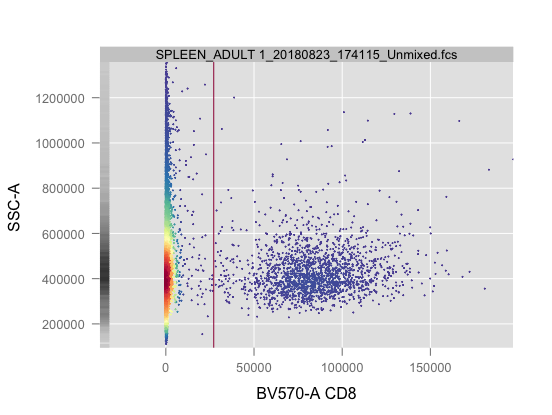
\includegraphics[width=0.6\linewidth]{/Users/monhait/Desktop/bookdown_autogating/images/cd8_data}

\hypertarget{transform-data-for-better-visualization}{%
\subsection{Transform data for better visualization}\label{transform-data-for-better-visualization}}

Although data will not be altered in any way, transformation may allow for better visualization. The most common form of transformation for flow cytometry analysis is \href{http://docs.flowjo.com/vx/graphs-and-gating/gw-transform-overview/}{biexponential}. Below is a comparison of gates without transformation and gates that have been transformed.

\textbf{Without Transformation}

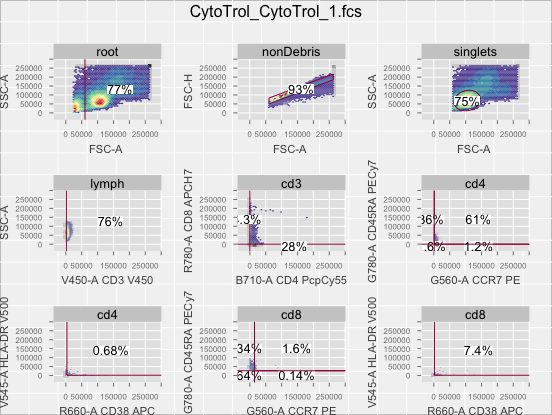
\includegraphics[width=0.6\linewidth]{/Users/monhait/Desktop/bookdown_autogating/images/no_trans}

\textbf{Transformed}

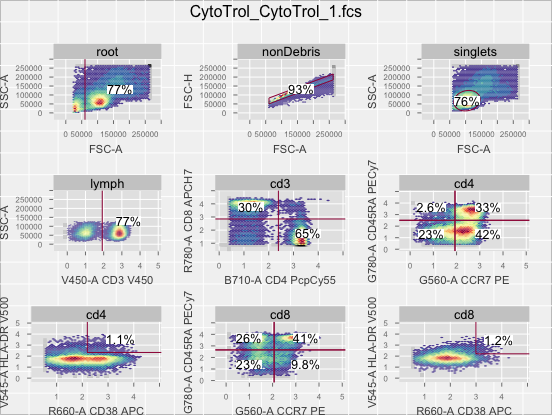
\includegraphics[width=0.6\linewidth]{/Users/monhait/Desktop/bookdown_autogating/images/trans}

\hypertarget{appendix}{%
\chapter{Appendix}\label{appendix}}

\hypertarget{function-and-r-object-definitions}{%
\section{Function and R Object Definitions}\label{function-and-r-object-definitions}}

\begin{tabular}{c|c}
\hline
Function/Object Name & Definition\\
\hline
wsfile & flowJo .wsp file location\\
\hline
openWorkspace() & function used to read in **wsfile**\\
\hline
ws & read in data from flowJo\\
\hline
parseWorkspace() & function to extract FCS files from **ws**\\
\hline
gating\_set & parsed FCS files to be gated\\
\hline
clone() & function used to create a clone of **gating\_set**\\
\hline
gh & subset of gating\_set\\
\hline
gt & .csv gating template\\
\hline
templateGen() & function used to generate a .csv template from existing manual gates\\
\hline
gatingTemplate() & function used to read in .csv template\\
\hline
gating() & function used to apply gates to a gating set\\
\hline
plot() & function to visualize gating tree\\
\hline
plotGate() & function to visualize gates\\
\hline
\end{tabular}


\end{document}
